\begin{tutorial}{Контейнеры}

\begin{center}
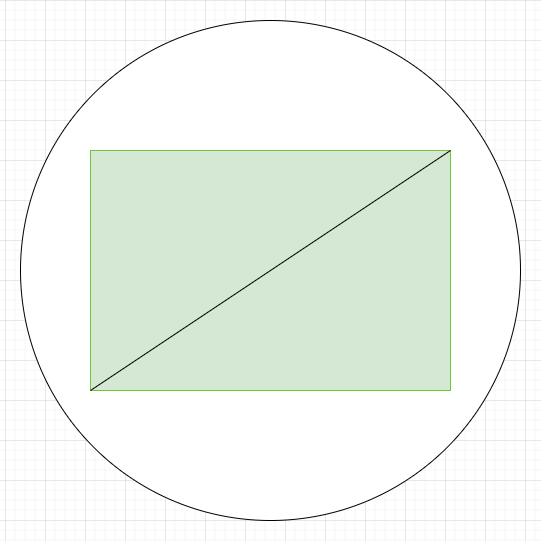
\includegraphics[width=4cm]{1.png}
\end{center}

Для каждого контейнера с помощью теоремы Пифагора вычисляем диагональ контейнера.

Контейнер помещается в круглый, люк если диагональ контейнера меньше, чем его диаметр.

\end{tutorial}
